\documentclass[fleqn]{article} % document instead of article?
\usepackage[T1]{fontenc}
\usepackage{ocgx2} %implements PDF Layers
\usepackage[colorlinks, urlcolor=blue, linkcolor=black]{hyperref}
\usepackage[inline]{enumitem}
\usepackage{amsmath}
\usepackage{amsfonts}
\usepackage{ulem}
\usepackage[a4paper, total={400pt, 10in}]{geometry}
\usepackage{tabto}
\usepackage{graphicx}
\usepackage{textcomp}
\usepackage{gensymb}
\usepackage{wrapfig}
\usepackage{svg}
\usepackage{multimedia}
\usepackage{esvect}
\usepackage[export]{adjustbox}
\usepackage{mathtools}  
\mathtoolsset{showonlyrefs}

\newenvironment{exercises}{\begin{enumerate*}[label=\alph*), itemjoin=\qquad]}{\end{enumerate*}}

\DeclareMathOperator{\tg}{tg}
\DeclareMathOperator{\ctg}{ctg}
\DeclareMathOperator{\arctg}{arctg}
\DeclareMathOperator{\arcctg}{arcctg}

\DeclareMathOperator{\jei}{\ jei\ }
\DeclareMathOperator{\ir}{\ ir\ }
\DeclareMathOperator{\arba}{\ arba\ }

\graphicspath{ {./assets/} }
% \title{Matematikos formulės}
% \author{Augustinas}
\begin{document}
% \maketitle

\renewcommand{\tablename}{Lentelė}
\renewcommand{\figurename}{Iliustracija}
\renewcommand{\vec}{\vv}
\pagestyle{plain}
\texttt{}

\hbadness=10001

\section{Būtina žinoti}

\subsection{Lygtys su vienu nežinomuoju}
$2x = x + 4$, $2x - x = 4$, $x = 4$ \\
Lygtyse, kai kintamasis pakeltas pirmuoju laipsnio rodikliu, kintamieji ir skaičiai turėtų būti skirtingose $=$ pusėse:
$x + 2 - 4x + 10 = 0$, $-3x = -12$, \\
Kitose lygtyse, kai kintamojo laipsnis $ > 1$, lygtį reikia prilyginti $0$.
\begin{equation}    
\begin{aligned}
    & (x - 4)^2 = 12 \\
    & x^2 - 8x + 16 = 12 \\
    & x^2 - 8x + 4 = 0 \dots
\end{aligned}
\qquad
\begin{aligned}
    & x(x - 4) = 0 \\
    & x = 0\arba x - 4 = 0 \\
    & x = 0\arba x = 4    
\end{aligned}
\qquad
\begin{aligned}    
    % & (x + 3)(x + 4) = 0 \\
    % & x + 3 = 0\arba x + 4 = 0 \\
    % & x = -3\arba x = -4
    & x^4 + 81 = 0 \\
    & \sqrt[4]{x^4} = \sqrt[4]{81} \\
    & x = 3 \arba  x = -3
\end{aligned}
\end{equation}

\begin{equation}
    ax^2 + bx + c = 0, \\
    D = b^2 - 4ac,     \\
    x = \frac{-b \pm \sqrt{D}}{2a}
\end{equation}


\section{Skaičių aibės}
Aibė -- nesikartojančių daiktų (dažniausia skaičių) rinkinys.
\begin{equation}
\{1; 2; -3; 3.5; \pi\}
\end{equation}

\begin{table}[h]
\begin{tabular}{c|l|l}
    
    Simb. & Reikšmė                                 & Aibės nariai/elementai \\
    \hline
    $\mathbb{N}$ & Visų natūraliųjų skaičių aibė    & $\{1; 2; 32768\:\dots\}$ \\
    $\mathbb{Z}$ & Visų sveikųjų skaičių aibė       & $\{-1; 0; 1\:\dots\}$ \\
    $\mathbb{Q}$ & Visų racionaliųjų skaičių aibė   & $\{\frac{1}{4}; -\frac{1}{16}\:\dots\}$ \\
    $\mathbb{I}$ & Visų iracionaliųjų skaičių aibė  & $\{-\pi; \sqrt{2}\:\dots\}$ \\
    $\mathbb{R}$ & Visų realiųjų skaičių aibė       & $\mathbb{Q} \cup \mathbb{I}$ \\
                 & Visų pirminių skaičių aibė       & $\{2; 3; 5; 7; 13 \dots \}$ \\
                 & Visų sudėtinių skaičių aibė      & $\{4; 6; 8; 9; 10\dots\}$ \\
    $\phi$       & Tuščia aibė                      &
\end{tabular}
\caption[Dažnai naudojamos aibės]{Dažnai naudojamos aibės}
\label{table:data}
\end{table} 

\begin{table}[h]
    \begin{tabular}{c|l|l}
        
        Simb. & Reikšmė                             & Pavyzdys \textit{(-iai)} \\
        \hline
        $\cup$      & Aibių sąjunga                 & $\{1; 2\} \cup \{2; 3\} = \{1; 2; 3\}$ \\
        $\cap$      & Aibių sankirta                & $\{1; 2\} \cap \{2; 3\} = \{2\}$ \\
        $\setminus$ & linktarget{Aibių skirtumas}   & $\{1; 2\} \setminus \{2; 3\} = \{1\}$ \\
        $\subset$   & Poaibis                       & $\{1; 2\} \cup \{2; 3\} = \{1; 2; 3\}$ \\
        $\in$       & Priklauso                     & $2 \in \{1; 2; 3\}$, $\{1; 2\} \in \{\{1; 2\}; 3\}$ \\
    \end{tabular}
    \caption[Veiksmai su aibėmis]{Veiksmai su aibėmis}
\end{table} 

\begin{align}
    \mathbb{N} \in \mathbb{Z} \in \mathbb{Q} & \in \mathbb{R} \in \dots \\
    \mathbb{I} & \in \mathbb{R} \\
    \mathbb{Q} \cup \mathbb{I} & = \mathbb{R}
\end{align}

\subsection{Pratimai}

Kokiai mažiausiai, iš čia išvardintų, aibių \uwave{priklauso}: \\
\begin{exercises}
    \item $5$
    \item $1.3$
    \item $\{1; 2; 2\pi\}$
    \item $\left[0; 1\right]$ 
    \item $\frac{1}{x}, x \in \mathbb{N}$ 
\end{exercises} 

\subsection{Daugiau}

\href {https://en.wikipedia.org/wiki/Set-theoretic_definition_of_natural_numbers}{[EN] Natūraliųjų skaičių apibrėžimas aibių/setų teorijoje.}

\section{Dešimtainės begalinės periodinės trupmenos} 
$1,36(24) = 1,3624242424242424 \dots$ arba \\
\textit{Vienas sveikas, 36-ios šimtosios ir 24-ios dešimttūkstantosios periodu.}

\begin{equation}
    \begin{aligned}
        x       &= 0,(2)        \\
        10x     &= 2,(2)        \\
        10x - x &= 2,(2) - 0,(2)\\
        9x      &= 2            \\ 
        x       &= \frac{2}{9}
      \end{aligned}
      \qquad
      \begin{aligned}
        x         &= 0,5(24)            \\
        100x      &= 52,(42) = 52,4(24) \\
        100x - 1x &= 52,4(24) - 0,5(24) \\ 
        99x       &= 51,9               \\
        x         &= \frac{519}{990} 
      \end{aligned}
  \end{equation}


\subsection{Pratimai}

Paverskite šias dešimtaines trupmenas į paprastąsias: \\
\begin{exercises}
    \item $2,5      $
    \item $9,(9)    $
    \item $6,(72)   $
    \item $330,(98) $
    \item $10,8(9)  $ 
\end{exercises} 

\begin{align*}
    x   &= -1,234(5)              \\
    10x &= -12,345(5)             \\
    9x  &= -12,345(5) - -1,234(5) \\
    9x  &= -11,111  \qquad  x = -\frac{11111}{9000}
\end{align*}  

\subsection{Daugiau}
$0$ sveikų, $\frac{9}{10}$ periodu yra lygu $1$:
\begin{math}\\
    0,(9) = 1, nes{:}\; 9,(9) - 0,(9) = 10x - 1x;\; 9x = 9;\; x = 1
\end{math}


\section{Logaritmai}

Logaritmas duoda laipsnio rodiklį, kuriuo pagrindas turėtų būti pakeltas, kad gautusi logaritmo argumentas.
$\log_a b = c,\;a^c = b$.

\begin{math}
    \log_a b = c, jei\; a > 0, a \ne 1, b > 0
\end{math}

\begin{itemize}
    \item $a \ne 1, nes \log_1 x = c,\,x = 1^c = 1,\, c \in \mathbb{R}\; 
    (c = 1 = a, c = 2 = a, c = -3 = a \dots)$
    \item $a > 0, nes \log_{-2} x = c, x = (-2)^c,\,jei\;c = \frac{a}{b}\;ir\;b - lyginis,\;o\;a - ne{:}\; (-2)^\frac{a}{b} = \phi,\\ \hspace*{10mm} pvz{:}\; (-2)^\frac{1}{2} = \sqrt{-2}, taigi{:}\;\log_{-2} \phi = \frac{1}{2}, nors{:}\; \log_{-2} 4 = 2$
    \item $b > 0, jei\;a > 0\;arba\;b - lyginis.$
\end{itemize}

\subsection{Logaritmų savybės}
\begin{itemize}
    \item $\log_a(xy) = \log_a x + \log_a y$
    \item $\log_a(\frac{x}{y}) = \log_a x - \log_a y$
    \item $\log_a(x^k) = k\log_a x$
    \item $\log_a b = \frac{\log_c b}{\log_c a}$\qquad $(\log_a \rightarrow \log_c)$
    \item $a^{\log_a b} = b$
\end{itemize}

\subsection{Pratimai}

\begin{exercises}
    \item $\log_2(8)            $
    \item $\log_4(64)           $
    \item $\log_3\,x = 3        $
    \item $\log_2 6 + \log_2 4  $
    \item $8\log_4 2           $
    \item $\log_4(x) + 1 = 3    $
\end{exercises} 

\subsection{Daugiau}

$\log_{10} x$ arba $\lg x$ gali duoti argumento skaitmenų skaičių: $\lfloor log_{10} x \rfloor + 1$. \\
$\frac{log_e x}{log_e a} = log_a x$ duodą log su norimu pagrindu. $\frac{log_e 64}{log_e 4} = 3$.

\section{Šaknys}
\begin{math}
    \sqrt{a} * \sqrt{b} = \sqrt{a * b} \\
    (\sqrt{a})^n = \sqrt{a^n} \\
    \sqrt[n]{\sqrt[k]{a}} = \sqrt[n * k]{a} \\
    \sqrt[2n]{a} = |a| = \{a; -a\}, \sqrt[2n + 1]{a} = a \\
    a^{\frac{n}{k}} = \sqrt[k]{a^n}
\end{math}

\section{Raidiniai reiškiniai}

\begin{math}
    (a - b)(a + b) = a^2 + b^2 \\
    (a \pm b)^2 = a^2 \pm 2ab + b^2 \\
    (a \pm b)^3 = a^3 \pm 3a^2b + 3ab^2 \pm b^3 \\
    (a \pm b)(a^2 \mp 1ab + b^2) = a^3 \pm b^3
\end{math}

\subsection{Pratimai}

\begin{exercises}
    \item $\log_2(8)                         $
    \item $x(x + 1)                          $
    \item $(x - y)(x - y)                    $
    \item $\frac{2}{x - y} + \frac{x + y}{1} $
    \item $\frac{x^2 - y^2}{x + y}           $
    \item $(\frac{x + y}{\sqrt{x + y}})^2$
\end{exercises} 

\section{Moduliai}

\[
|x| =
\begin{cases}
    x,  &kai\ x \ge 0, \\
    -x, &kai\ x < 0
\end{cases}     
\]

\[
|x| + 2 = 4 \qquad
|x| = 2     \qquad
x = 2\ arba\ x = -2,\ nes \qquad
|2| = 2\ ir\ |-2| = 2
\]


Lygtį $|-x + 5| = 4$ galima išspręsti taip:
\begin{equation}
    \begin{aligned}
        5 - x &= 4 \\
        -x &= -1 \\
        x &= 1\ (Tinka) \\
        |-1 + 5| &= 4
    \end{aligned}
    \hspace{10mm}
    \arba
    \hspace{10mm}
    \begin{aligned}
        x - 5 &= 4 \\
        x &= 9\ (Tinka) \\
        |-9 + 5| &= 4
    \end{aligned}    
\end{equation}


\section{Lygčių sistemos}

Lygtis su dviem nežinomaisiais galima išspręsti grafiškai \textit{(bet taip nespręskit)} sudėties ir keitimo būdu.

\subsection{Lygtys su dviem nežinomaisiais}
\begin{equation}
    \begin{cases}
        x + y &= 8, \\
        x - y &= -4
    \end{cases}
    \Rightarrow
    \begin{cases}
        x + y &= 8, \\
        x     &= y - 4
    \end{cases}
    \Rightarrow
    \begin{cases}
        (y - 4) + y &= 8, \\
        x           &= y - 4
    \end{cases}
    \Rightarrow
    \begin{cases}
        y &= 6, \\
        x &= 2
    \end{cases}
\end{equation}

\begin{equation}
    \begin{cases}
        x + y = &= 8, \\
        x - y = &= -4
    \end{cases}
    \Rightarrow +
    \begin{cases}
        x + y = &= 8, \\
        x - y = &= -4 \\
        \hline
        2x &= 4 
    \end{cases}
    \Rightarrow
    \begin{cases}
        x = 2, \\
        y = 6
    \end{cases}
\end{equation}
\textit{Be to galima padauginti vieną lygtį(eilutę) iš $-1, -2, 3 \dots$} \\
\textbf{Sudėties metodas kartais neveikia, vienas iš kintamųjų TURI pradingti, sudėjus lygtis:}
\begin{equation}
    \begin{cases}
        x + y = 8 \\
        x\ \cdot\ y = -4  
    \end{cases}
    \Rightarrow +
    \begin{cases}
        x + y = 8 \\
        x\ \cdot\ y = -4 \\
        \hline
        x + y + xy = 4
    \end{cases}
    \Rightarrow
    x + y + xy = 4
\end{equation}

\subsection{Lygtys su trimis nežinomaisiais}
\begin{equation}
    \begin{cases}
        x + y + z &= 6 \\
        x - y + z &= 2 \\
        z - y - x &= 0
    \end{cases}
    \Rightarrow
    \begin{cases}
        x + y + z &= 6 \\
        x - y + z &= 2 \\
        z         &= x + y
    \end{cases}
    \Rightarrow
    \begin{cases}
        x + y + (x + y) &= 6 \\
        x - y + (x + y) &= 2 \\
        z &= x + y
    \end{cases}
\end{equation}
\begin{equation}
    \Rightarrow
    \begin{cases}
        2x + 2y &= 6 \\
        2x &= 2 \\
        z &= x + y
    \end{cases}
    \Rightarrow
    \begin{cases}
        x &= 1 \\
        y &= 2 \\
        z &= 3
    \end{cases}
\end{equation}
\textit{Čia sudėties būdas irgi galimas, tik jis veikia daug rečiau. Dažnai gali būti naudojamas mišrus būdas, dvi lygtis sudedame ir rezultatą (keitimo būdu) įstatome į trečią.}



\section{Trikampiai}

\subsection{Radianai}
Radianas - kampo dydžio matavimo vienetas. \textbf{Gali} būti žymimas: $rad$.

\begin{math} \\
    1rad = \frac{180}{pi}\degree \approx 57 \degree \\
    1\degree = \frac{pi}{180}
\end{math}

\subsection{Trigonometrinės funkcijos}
Trigonometrinės funkcijos yra $\sin$, $\cos$, $\tg$, $\ctg$, $\arcsin$ ir daugiau\dots
Jos gali būti naudojamos išmatuoti smailųjį kampą stačiajame trikampyje, daugelyje formulių ir t.t\dots

\subsection{Statieji trikampiai}
{
\begin{wrapfigure}{l}{0.4\textwidth}
\caption{\textit{Iliustracijos -- tiek reikalingos, kiek nuobodžios daryti.}}
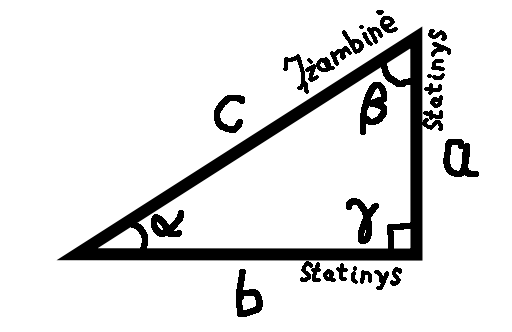
\includegraphics[scale=0.5]{right_triangle.png}
\end{wrapfigure}

\begin{equation*} \\
    \begin{aligned}[c]
        \sin \alpha &= \frac{a}{c} \\
        \cos \alpha &= \frac{b}{c} \\
        \tg  \alpha &= \frac{a}{b} \\
        \ctg \alpha &= \frac{b}{a}
    \end{aligned}
    \hspace{10mm}
    \begin{aligned}[c]
        c^2 &= a^2 + b^2 \\
        S &= \frac{ab}{2}
    \end{aligned}
\end{equation*}
}

\clearpage
\subsection{Įvairiakraščiai trikampiai}

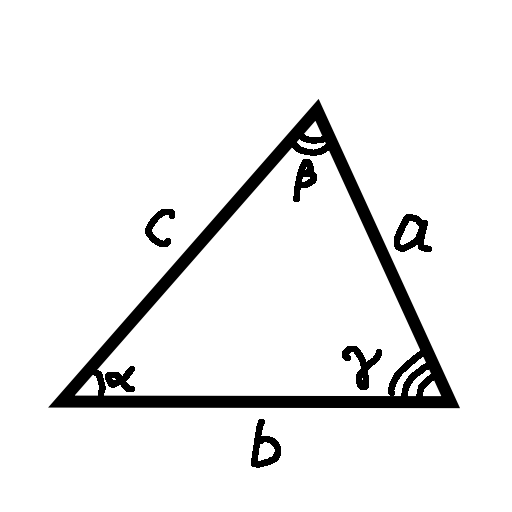
\includegraphics[scale=0.5]{icocele_triangle.png}

\begin{equation*}
    \begin{aligned}[c]
        180\degree &= \alpha + \beta + \gamma \\
        \frac{a}{\sin \alpha} &= \frac{b}{\sin \beta} = \frac{c}{\sin \gamma} \\
        a^2 &= b^2 + c^2 - 2\, b\, c\,\cos \alpha \\
        S &= \frac{a\,b}{2} \cdot \sin \gamma
    \end{aligned}
    \hspace{40mm}
    \begin{aligned}[c]
        \textit{Sinuso\ teorema} \\
        \textit{Kosinuso\ teorema} \\
    \end{aligned}
\end{equation*}


\subsection{Trigonometrinės formulės}

\begin{equation*} \\
    \begin{aligned}[c]
        \sin(\alpha \pm \beta) &= \sin\alpha\cos\beta \pm \sin\beta\cos\alpha \\
        \cos(\alpha \pm \beta) &= \cos\alpha\cos\beta \mp \sin\alpha\sin\beta \\
        \tg (\alpha \pm \beta) &= \frac{\tg\alpha \pm \tg\beta}{1 \mp \tg\alpha \tg\beta} \\ \\
        \sin(2\alpha) &= \sin(\alpha + \alpha) = 2\sin\alpha\cos\alpha \\
        \cos(2\alpha) &= \cos(\alpha + \alpha) = \cos^2\alpha - \sin^2\alpha
    \end{aligned}
    \hspace{20mm}
    \begin{aligned}[c]
        \sin{\alpha}^2 + \cos{\alpha}^2 &= 1 \\
        \tg \alpha \cdot \ctg \alpha &= 1 \\
        \tg \alpha &= \frac{\sin \alpha}{\cos \alpha} \\
        \ctg \alpha &= \frac{1}{\tg \alpha} \\
        1 + \tg^2 \alpha &= \frac{1}{\cos^2 \alpha} \\  
        1 + \ctg^2 \alpha &= \frac{1}{\sin^2 \alpha} \\  
    \end{aligned}
\end{equation*}

\subsubsection{Pratimai}

\begin{exercises} \\
    \item $\ctg 30\degree               $
    \item $\ctg(45\degree + 45\degree)  $
    \item $\sin 75\degree               $
    \item $\cos( \alpha - 90\degree )   $
    \item $\tg \alpha\ ((\tg\alpha\ (\tg \alpha + \ctg \alpha))^{-1}\ - 1) $ 
\end{exercises} 

\subsubsection{Daugiau}

\begin{math}
    \sin(10\cdot 30\degree) = \sin(30\degree + 9 \cdot 30\degree) = \\
    \sin 30\degree \cos 30\degree + \sin(9 \cdot 30\degree)\cos(9 \cot 30\degree) = \\
    \frac{\sqrt{3}}{4} + \sin(30\degree + 8 \cdot 30\degree)\cos(30\degree + 8 \cdot 30\degree) = ... \\ 
    \\
    \sin(10 \cdot 30\degree) = \sin(300\degree) \Rightarrow 
    \sin(300\degree - 270\degree) \Rightarrow -\cos(30\degree) = -\frac{\sqrt{3}}{2}
\end{math} \\

\begin{math} \\
    \tg(\alpha + \beta) = \frac{\sin(\alpha + \beta)}{\cos(\alpha + \beta)}
\end{math}

\subsection{Redukcija}

Redukcija yra naudojama norint gauti tikslią $\sin, \cos, \tg$ ar $\ctg$ reikšmę iš lentelės (kurioje visos reikšmes yra nuo $0$ iki $90\degree).$ \\

Trig. funkcijų periodai$(T)$: $T_{sin} = 360\degree, T_{cos} = 360\degree, T_{tg} = 180\degree, T_{\ctg} = 180\degree $

$\sin(\alpha + 90\degree) = \cos\alpha$
\begin{enumerate}
    \item Jei $\alpha > T$, \\
        $\alpha \Rightarrow \alpha \mod T$, \textit{arba atimti $T$ iš $\alpha$, kol $\alpha < T$}
    \item Jei $\alpha \ge 90\degree$, žiūrėti pagal ketvirčius: \\
        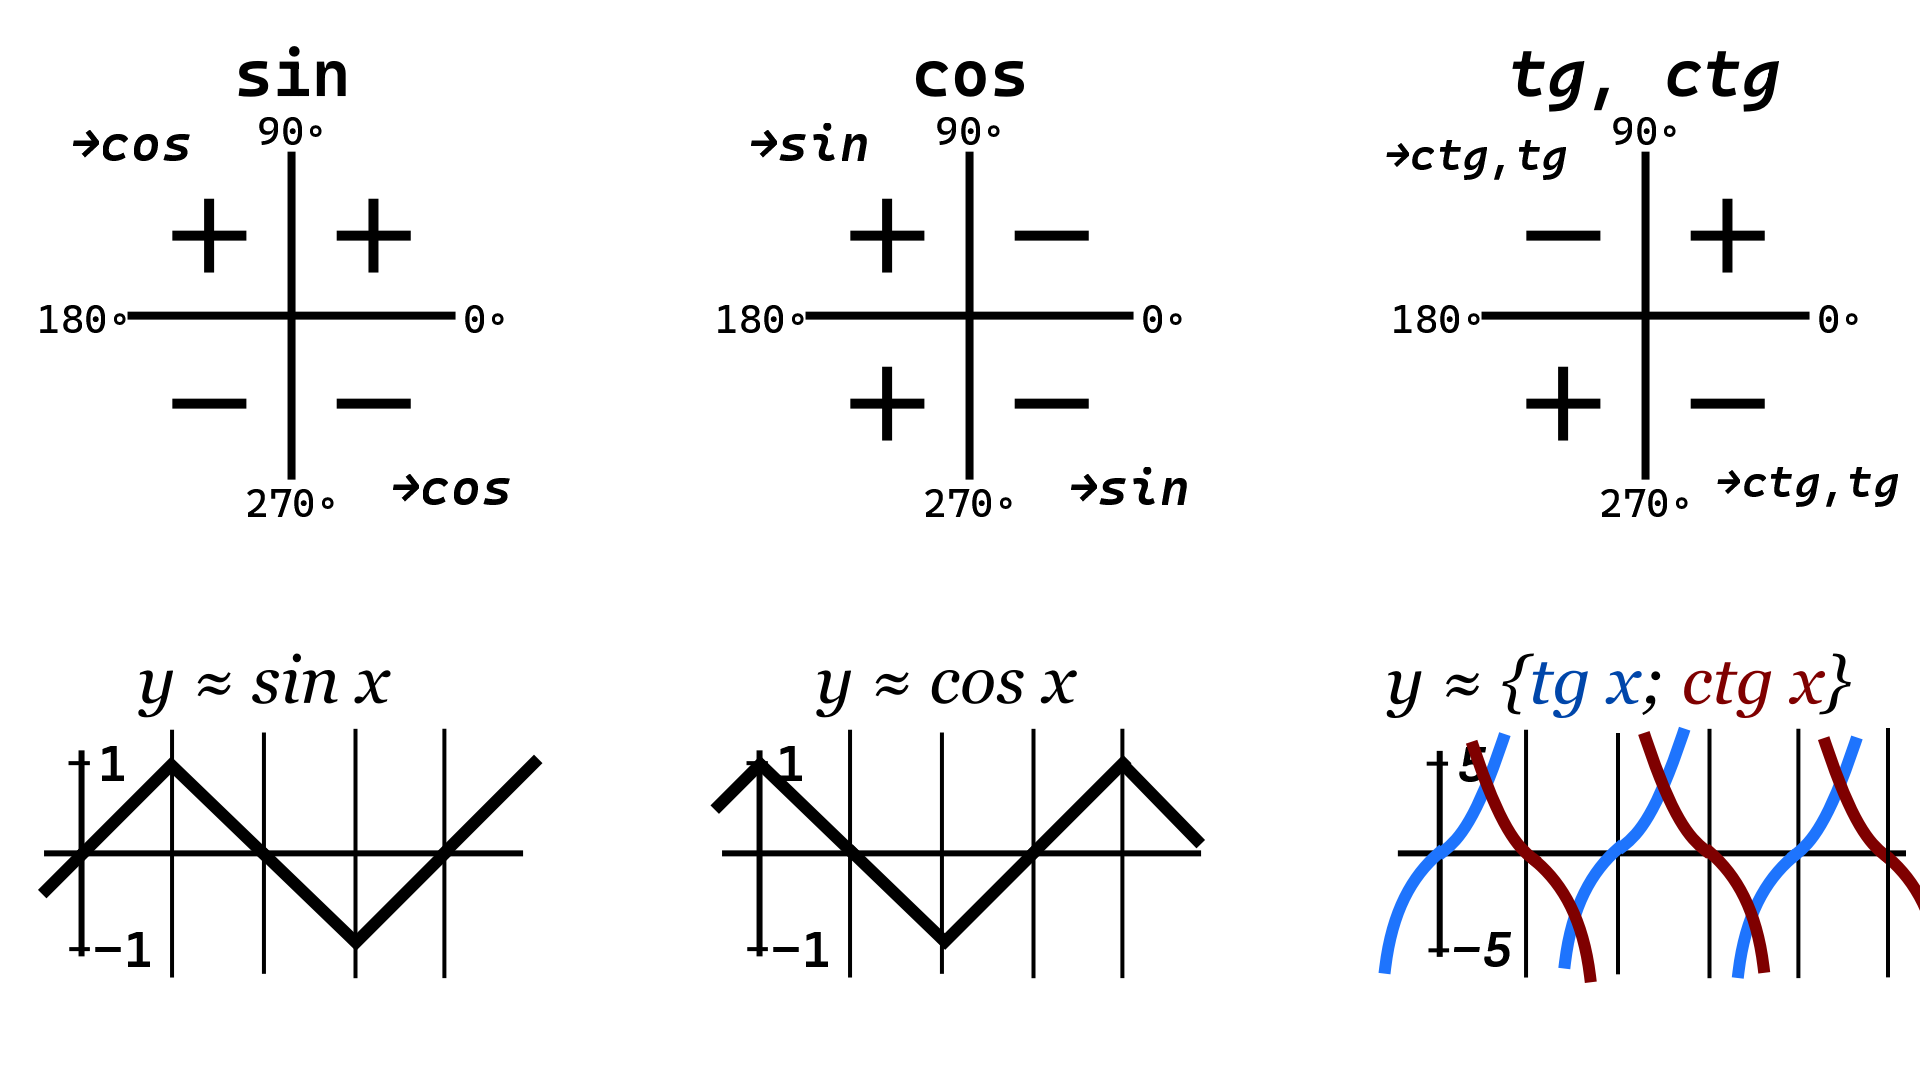
\includegraphics[scale=0.25]{assets/reduction.png} 
    \item Jei $\alpha \le 90\degree$, \\
        tikslią trig. funkcijos reikšmę galima rasti lentelėje.

\end{enumerate}

\subsubsection{Pratimai}

\begin{exercises}
    \item $\sin 30\degree         $
    \item $\cos 30\degree         $
    \item $\sin 270\degree        $
    \item $\tg  300\degree        $ 
    \item $\ctg 120\degree        $
    \item $\sin 720\degree n, n \in \mathbb{Z} $
    \item $\sin(-45\degree) $
\end{exercises} 


\subsubsection{Daugiau}

\begin{table}[h]
    \begin{tabular}{|c|ccccccccc|} 
        % There has got to be a better way to do this, but I don't care right now
        \hline
        $\alpha,\,\degree$ & 0 & 30 & 45 & 60 & 90 & 120 & 135 & 150 & 180 \\ 
        \hline
        $\sin \alpha$ & 0 & $\frac{1}{2}$ & $\frac{\sqrt{2}}{2}$ & $\frac{\sqrt{3}}{2}$ & 1 
                      & $\frac{\sqrt{3}}{2}$ & $\frac{\sqrt{2}}{2}$ & $\frac{1}{2}$ & 0 \\
        \hline
    \end{tabular}
    \\ \\ \\
    \begin{tabular}{|c|cccccccc|}
        \hline
        $\alpha,\,\degree$ & 210 & 225 & 240 & 270 & 300 & 330 & 345 & 360 \\ 
        \hline
        $\sin \alpha$ & $-\frac{1}{2}$ & $-\frac{\sqrt{2}}{2}$ & $-\frac{\sqrt{3}}{2}$ & -1
                      & $-\frac{\sqrt{3}}{2}$ & $-\frac{\sqrt{2}}{2}$ & $-\frac{1}{2}$ & 0 \\
        \hline
    \end{tabular}
    \caption{Pratęsta $\sin \alpha$ lentelė}
\end{table}


\subsection{Atvirkštinės trigonometrinės funkcijos (arc-funkcijos).}

\begin{equation}
    \begin{aligned}[c]
        \sin(\arcsin a) &= a, & \arcsin x &= y,\,kai\ -1 \le x \le 1\ ir\ y \in \left[ -\frac{\pi}{2}; \frac{\pi}{2}\right] \\
        \cos(\arccos a) &= a, & \arccos x &= y,\,kai\ -1 \le x \le 1\ ir\ y \in \left[0;\pi\right] \\
        \tg (\arctg  a) &= a, & \arctg  x &= y,\,kai\ y \in \left[ -\frac{\pi}{2}; \frac{\pi}{2}\right]\\
        \ctg(\arcctg a) &= a, & \arcctg x &= y,\,kai\ y \in \left[0;\pi\right]
    \end{aligned}
\end{equation}

\begin{equation}
    \begin{aligned}[c]
        \sin x &= y, & x &= (-1)^n + \arcsin y + \pi{n}, n \in \mathbb{Z} \\
        \cos x &= y, & x &= \pm \arccos y + 2\pi{n}, n \in \mathbb{Z} \\
        \tg  x &= y, & x &= \arctg y + \pi{n}, n \in \mathbb{Z} \\
        \ctg x &= y, & x &= \arcctg y + \pi{n}, n \in \mathbb{Z} \\
    \end{aligned}
\end{equation}

\begin{equation}
    \left.
    \begin{aligned}[c]
        \sin x &= -1, & x &= -\frac{\pi}{2} &+\ 2\pi{n} \\
        \sin x &=  0, & x &=                &    \pi{n} \\
        \sin x &=  1, & x &= +\frac{\pi}{2} &+\ 2\pi{n}
    \end{aligned}
    \hspace {15mm}
    \begin{aligned}[c]
        \cos x &= -1, & x &= \pi            &+\ 2\pi{n} \\
        \cos x &=  0, & x &= \frac{\pi}{2}  &    \pi{n} \\
        \cos x &=  1, & x &=                &+\ 2\pi{n}
    \end{aligned}
    \hspace{5mm}
    \right\}
    n \in \mathbb{Z}
\end{equation}

\subsubsection{Daugiau}

$\arcsin x = y$, $y \in [-\frac{\pi}{2}; \frac{\pi}{2}]$, o ne, pavyzdžiui: $y \in [-\pi; \pi]$, nes y tūrėtų 2 atsakymus, būtų aibė $y = \{x_1; x_2\}$.

% \includegraphics[scale=0.5]{assets/arcsin_restriction_reason.png} TODO, oops

\section{Kitos Figūros}

\textit{Vėliau padarysiu...}

\section{Vektoriai}

Skaliaras - vienas skaičius. \textit{Angl. scalar, scale} \\
Vektorius - skaliarų sąrašas, pavyzdžiui: $\{x; y; z; 40, 50\}$. Vektorius galima pavaizduoti plokštumoje naudojant atkarpą.

\begin{table}[h]
    \begin{tabular}{rll}
        Skaliaras & $a$ \\
        Vektorius & $\{a_1; a_2 \dots a_n\}$\\
        Matrica   & $\begin{bmatrix}
            a_1 & a_2 & \dots & a_n \\
            b_1 & b_2 & \dots & b_n \\
            \dots & \dots & \dots & \dots
        \end{bmatrix}$ \\
        \dots & \dots
    \end{tabular}
    \hspace{40mm}
    \begin{tabular}{rc}
        Ašis & Pavadinimas \\ \hline
        OX & Abscisių ašis \\
        OY & Ordinačių ašis \\
        OZ & Aplikačių ašis
    \end{tabular}
\end{table}
Mes naudojame vektorius, kurie turi: $\{x; y\}$ arba $\{x; y; z\}$. Pavyzdžiui: $\vec{AB}(3;\,4)$.

\begin{wrapfigure}{l}{0.4\textwidth}
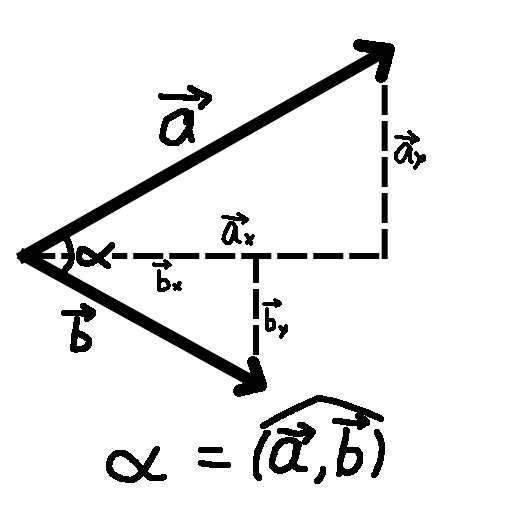
\includegraphics[scale=0.4]{vector_basics.png}
\end{wrapfigure}

\begin{equation}
    \hspace{10mm}
    \begin{aligned}
        \vec{AB} & (x_2 - x_1; y_2 - y_1; z_2 - z_1) \\
        \vec{i} & (1, 0, 0), \vec{j}(0, 1, 0), \vec{k}(0, 0, 1) \\
        \vec{AB} &= (x_2 - x_1) \cdot \vec{i} + (y_2 - y_1) * \vec{j} + (z_2 - z_1) \cdot \vec{k} \\
        |\vec{AB}| &= \sqrt{x^2 + y^2 + z^2} \\
        \vec{AB} + \vec{BC} &= \vec{AC} \ne \vec{CA} \\
        \vec{AB} - \vec{BC} &= -\vec{AC} = \vec{CA} \\
        \vec{a} \cdot n &= \vec{a} + \vec{a} + \dots \}\ n \text{ kartų} \\
        \vec{a} \cdot \vec{b} &= |\vec{a}| \cdot |\vec{b}| \cdot \cos{\widehat{(\vec{a}; \vec{b})}} \\
        \vec{a} \cdot \vec{b} &= \vec{a}_x \cdot \vec{b}_x + \vec{a}_y \cdot \vec{b}_y \\
        \vec{a} \cdot \vec{b} &= \frac{\vec{a} \cdot \vec{b}}{|\vec{a}||\vec{b}|}
    \end{aligned}
\end{equation}

\begin{table}[h]
    \begin{tabular}{rcl}
        Vektoriaus tipas& Pavyzdžiai & Apibrėžimas \\ \hline
        Kolinearieji    & \includegraphics*[scale=0.25]{colinear_vectors.png} & $\vec{a}_x : \vec{b}_y = \vec{a}_x : \vec{b}_x$ \\
        Vienkrypčiai    & \includegraphics*[scale=0.25]{one-way_vectors.png} & $\vec{a} \uparrow \uparrow \vec{b}, \vec{a} \cdot m = \vec{b}, m > 0$  \\
        Priešpriešiniai & \includegraphics*[scale=0.25]{opposite-facing_vectors.png} & $\vec{a} \uparrow \downarrow \vec{b}, \vec{a} \cdot m = \vec{b}, m < 0$ \\
        Statmeni        & \includegraphics*[scale=0.25]{perpendicular_vectors.png} & $\vec{a} \perp \vec{b}, \;\vec{a} \cdot \vec{b} = 0 $ \\
        Lygieji         & \includegraphics*[scale=0.25]{equal_vectors.png} & $\vec{a} = \vec{b}$ \\
        Priešingieji    & \includegraphics*[scale=0.25]{opposite_vectors.png} & $\vec{a} = -\vec{b}$ \\
        Nulinis         & $\vec{AA}$ & $|\vec{a}| = 0$
    \end{tabular}
\end{table}

\clearpage

\subsection{Vektorių sudėtis}
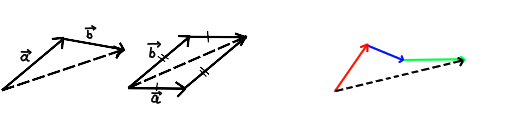
\includegraphics{assets/vector_addition.png}

\subsubsection{Pratimai}

Išreiškite vektorius, kuriuos reikėtų sudėti, kad gautumėte $\vec{AZ}$

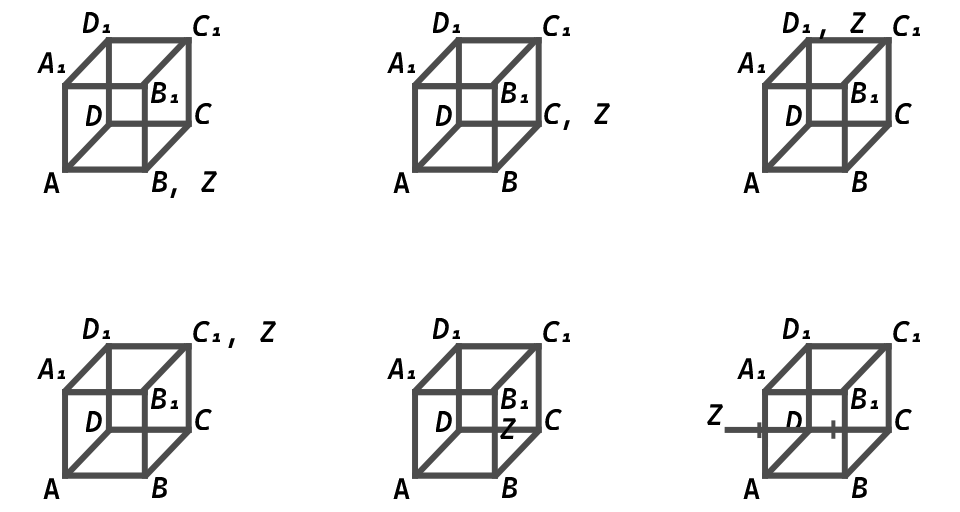
\includegraphics[max width=\textwidth]{assets/vector_exercise.png}
Raskite dydžius, kai A(10; 11), B(7; 7), C(4, 1), D(15, 13): \\
\begin{exercises}
    \item $|\vec{AB}|                           $
    \item $\vec{AB} + \vec{CD}                  $
    \item $\vec{AD} \cdot 2                     $
    \item $\vec{AB} \cdot \vec{CD}              $
    \item $\frac{\vec{AB}}{\vec{CD}}            $
    \item $\cos \widehat{(\vec{AB}, \vec{DC})}  $
\end{exercises}

\subsubsection{Daugiau}

$\vec{a} \ne (\vec{a}_x; \vec{a}_y)$, nes $(a_1, a_2 \dots )$ yra sekos sintaksė.

\clearpage

\section{Geometrija}

\subsection{Kampai}

\begin{equation}
    \text{Visų figūros kampų suma} = (n - 2) \cdot 180\degree,\ n - \text{kampų skaičius}
\end{equation}

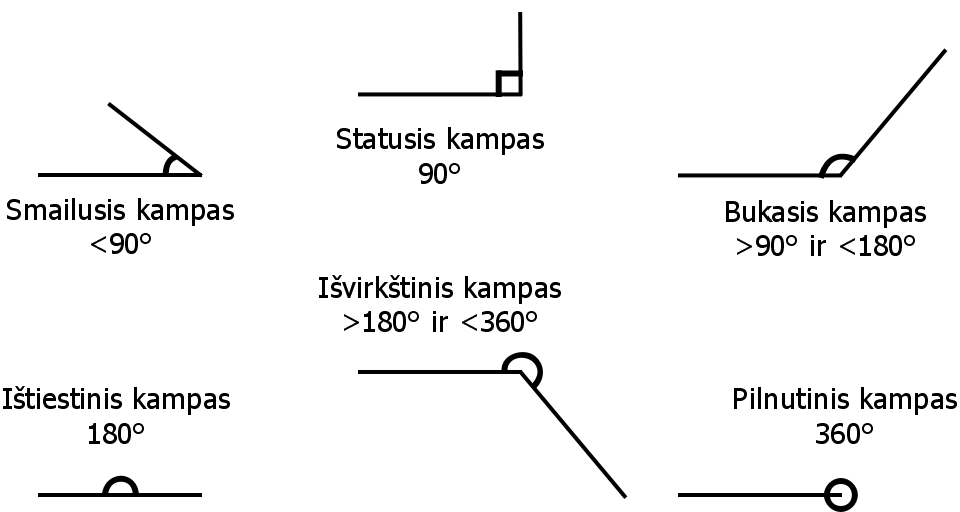
\includegraphics[max width=\textwidth]{assets/angle_types.png}

\subsection{Įbrėžtinės ir Apibrėžtinės figūros}

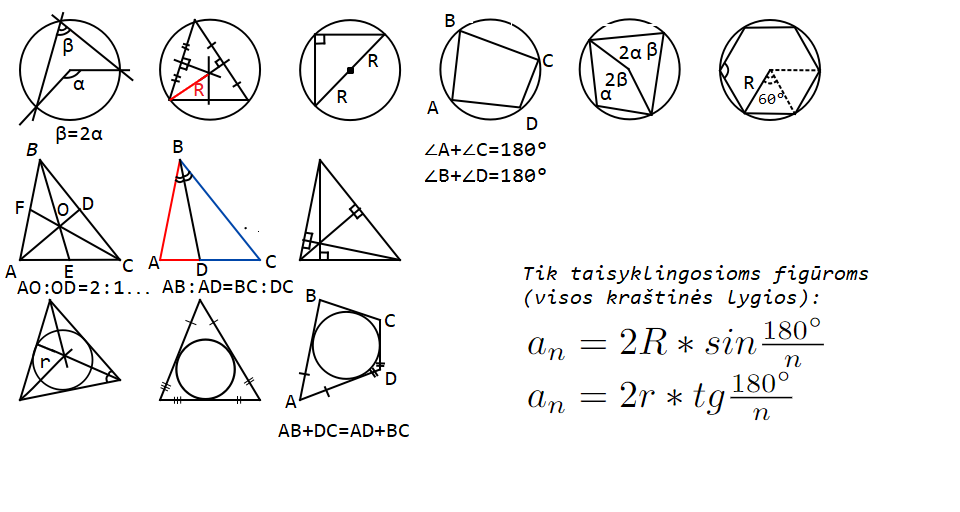
\includegraphics[max width = \textwidth]{assets/geometry.png}

\section{Daugiau}

Apskritimas gali būti vaizduojamas kaip lygtis su dviem kintamaisiais:
\[
    (x - O_x)^2 + (y - O_y)^2 = r^2,\ r > 0 \\ 
    O - \text{apskritimo centro taškas, } O(x, y)
\]

\subsection{Lygties sprendimas įvedant naują kintamąjį}

\begin{align*}
    \begin{aligned}
    ax^4 + bx^2 + c = 0                 \\
    \jei t = x^2,                       \\
    at^2 + at + c = 0                   \\
    x_1 = \sqrt{t}, x_2 = -\sqrt{t}     
    \end{aligned}
    \qquad\qquad\qquad
    \begin{aligned}
    a\log^2_p x + b\log_p x + c = 0     \\
    \jei t = \log_p x,                  \\
    at^2 + at + c = 0                   \\
    x = p^t
    \end{aligned}
\end{align*}

$\log_p x, p - pagrindas$, \textit{man nebe užteko raidžių :(, $z$ -- ne, $d$ -- negraži, o $\log_e$ yra natūrinis logaritmas(Angl. natural logarithm)}\dots

\section{12 Klasė}

\section{Sekos}

Seka - tai, tiesiog, skaičių, kurie turi savo numerį/indeksą, sąrašas. 
Seka gali būti išreikšta: 
\begin{itemize}
    \item Pagal kiekvieną skaičių: $10, 20, 30, 40 \dots$
    \item n-ojo nario formule: $a_n = n \cdot 10, n \in \mathbb{N}$
    \item rekurentiškai: $a_1 = 10, a_{n + 1} = a_n + 10, n \in \mathbb{N}$
\end{itemize}
\textit{Sekos indeksas turi būti natūralus skaičius!}

\subsection{Aritmetinė progresija}
Aritmetinės progresijos yra sekos sekančios: $a_n = a_1 + (n - 1)d$ formulę. \\
$a_1$ -- pirmas sekos narys, $n$ -- nario numeris, $d$ -- skirtumas, $S$ -- suma.
\begin{align*}
    \begin{aligned}
    a_1 &= a_n - (n - 1)d \\
    n   &= \frac{a_n - a_1}{d} + 1 \\
    d   &= \frac{a_n - a_1}{n - 1} = a_{n + 1} - a_n \\
    \end{aligned}
    \quad\quad\quad
    \begin{aligned}
    S_n &= \frac{a_1 + a_n}{2}n = \frac{2a_1 + (n-1)d}{2} n \\
    a_{\frac{x + y}{2}} &= \frac{a_{x} + a_{y}}{2},\ (Vidurkis)
    \end{aligned}
\end{align*}

\subsection{Geometrinė progresija}

Geometrinės progresijos yra sekos sekančios: $b_n = b_1 q^{n - 1}$ formulę. \\
$b_1$ -- pirmas sekos narys, $n$ -- nario numeris, $q$ -- vardiklis, $S$ -- suma.
\begin{align*}
    \begin{aligned}
    b_1 &= b_n : q^{n - 1} \\
    n   &= \log_q{(\frac{b_n}{b_1} + q)} \\
    q   &= (\frac{b_1}{b_n})^{n - 1} = \frac{b_{n + 1}}{b_n} \\
    \end{aligned}
    \quad\quad\quad
    \begin{aligned}
    S_n &= \frac{b_1 - b_n q}{1 - q} = \frac{b_1(1 - q^n)}{1 - q} \\
    S   &= \frac{b_1}{1 - q} \\
    a_{\frac{x + y}{2}} &= \sqrt{a_{x} + a_{y}},\ (Vidurkis)
    \end{aligned}
\end{align*}


\subsection{Mišrių progresijų uždaviniai}
\textcolor{red}{Sėkmės.}

\subsection{Daugiau}
Kiek mačiau, Amerikoje beveik visad Aritmetinė ir Geometrinė progresijos sutrumpinamos į $AP$ ir $GP$.

\section{Nelygybės}
\subsection{Tiesinės nelygybės}
\subsection{Kvadratinės nelygybės}
\subsection{Trupmeninės nelygybės}
\subsection{Rodiklinės nelygybės}
\subsection{Logaritminės nelygybės}
\subsection{Modulinės nelygybės}
\subsection{Trigonometrinės nelygybės}


\section{Dar daugiau}

\subsection{Įsivaizduojamieji skaičiai($\mathbb{C}$):}
Šie skaičiai turi tikrają ir įsivaizduojamają dalis. Atrodo taip: $-12 + 2i$.
Tikroji dalis yra paprastas skačiius, be vieneto, kol įsivaizduojamoji turi $i$. Jei jums patinka, galite $i$ laikyti: $obuolys$ arba $knyga$... \\
Nors, svarbiausia: $i = \sqrt{-1}$ ir $i^2 = -1$. \\
Šie skaičiai taip pat veikia kaip plokštumos(2D) vektoriai, su kuriais daug lengviau daryti algebrą. Galite laikyti tikrają skaičiaus dalį $\vec{a}_x$ komponentu ir netrikrają $\vec{a}_y$ komponentu. \\
Beje, $\vec{i}(1, 0, 0 \dots )$ ir $\vec{j}(0, 1, 0 \dots)$ tai vienetiniai vektoriai!



\subsection{Sudėties apibrėžimas:}
\begin{math}
    3^2 = 3 * 3 = 3 + 3 + 3 = ? \\
    \\
    Jei\ a + 0 = a, a^+ = a + 1, \\
    a + 1 = a + 0^+ = (a + 0)^+ = a^+ \\
    a + b = a^{+\ \}b \text{ kartų}}
\end{math} 

\end{document}

% Todo:
%   - Probability?
%   - 
%
%